\graphicspath{{./images/Appendix/Comparison_Tools/}}
\chapter{Comparison of Tools}
\label{ch:app_comp_tools}
\paragraph*{\textnormal{In order to develop an extension for extending CPN with relational database, we decided to choose a tool for our development. We discussed few potential candidate tools for the CPN extension. A database which lists all the available tools for PNs/CPNs is available at \cite{Tools_WIKI}. We wanted to develop the extension in a well known programming language such as Java, C, C++ etc. Potential tools such as Renew \cite{Renew_Paper} and CPN Tools, came up. CPN Tools is one of the most popular tool for modelling, simulating and verifying CPNs and is also used in industry\cite{CPN_Industrial_Use}. Kurt Jensen, first talked about CPN, in his paper \cite{Jensen2007} and also in his book \cite{Jensen_CPN_Book_ML} talks about modelling with CPN Tools. With the known popularity of CPN Tools, we decided to pick this tool for the development purpose along with Renew.}}

\begin{comment}
\paragraph*{\color {red}\textnormal{In this chapter, we will discuss about CPN Tools and Renew. The first part provides an introduction to Renew, whereas the second part gives an introduction of CPN Tools. Later, we compare the tool on few parameters and justify our selection of the tool for the development our extension. This chapter is intentionally made short. If the reader is interested in details, then one can follow the mentioned references.}}
\end{comment}

\section{Renew (The Reference NetWorkshop)}
\label{sec:app_comp_tools_renew}
\paragraph*{\textnormal{From \cite{Renew_Paper}, Renew is an extensible Petri net IDE that supports the development and execution of high-level Petri nets and other modelling techniques. One of the most attractive feature of Renew is implementation language, JAVA, which makes developing extensions easier (since it is one the well known programming language). The reference net formalism in Renew combines the concept of nets-within-nets with a reference semantics. Nets-within-nets simply builds a hierarchical structure of nets. Java being an object oriented language enhances its expressive power. Renew also has the support for Object-oriented PNs, Place/Transition Nets and Timed PNs.}}

\paragraph*{\textnormal{The first official release of Renew was in 1999. Since then TGI\footnote{Theoretical Foundations Group, Department of Informatics, University of Hamburg.} group has continuously developed it as a Petri net IDE. Renew allow modelling of Coloured Petri nets along with its simulation. Besides being a Petri net IDE, it also has plug-ins for other modelling techniques such as diagram from BPMN(Business Process Model Notation) or UML (Unified Modelling Language).}}
\subparagraph*{\textnormal{One of the main focus for the development of Renew is the simulation of reference nets. One of the approaches in software development with emphasis on distribution and concurrency is PAOSE\footnote{Petri Net-based agent-oriented software engineering \cite{DBLP:phd/de/Cabac2010}.}. In order to develop multi-agent applications (MAA), reference nets are used as implementation artifacts. So, in Renew we can also perform simulation, modelling, editing and debugging over a CPN model.}}

\subsection*{Modelling}

\subparagraph*{\textnormal{Figure \ref{fig:Comparison_Tools_Renew_Net_GCD} represents a CPN to find GCD (greatest common divisors) of numbers in Renew. The net contains 3 transitions, 2 places and 7 arcs. Places $P1$ and $P2$ are of type \textit{int}. The initial marking of $P1$ consists of 3 integers 105, 60 and 42. The variables in the arc expression are declared as integers (in the right most side of the figure). In Renew, the guards on transitions are defined with the prefix keyword \bdq{guard}(see transition \textit{T2}). The role of \textit{T1} is to eliminate a token of data value 0 from the place \textit{P1}. The role of the transition \textit{T2} is to take two integers from \textit{P1}, calculate their remainder and divisor and forward it to the place \textit{P2}. The transition \textit{T3} establishes a loop by transferring tokens from \textit{P2} to \textit{P1}. The process terminates when there is only one element left at place \textit{P1} and this is the resultant GCD of the tokens present at the initial state.}}

\subparagraph*{\textnormal{The net structure can be drawn with the tools provided in the tool box. For names, inscriptions and declaration of the net elements, separate tools are provided. The colour/type of the places can be declared by just writing the JAVA type beside the places.}}

\begin{figure}[!htbp]
	\centering
	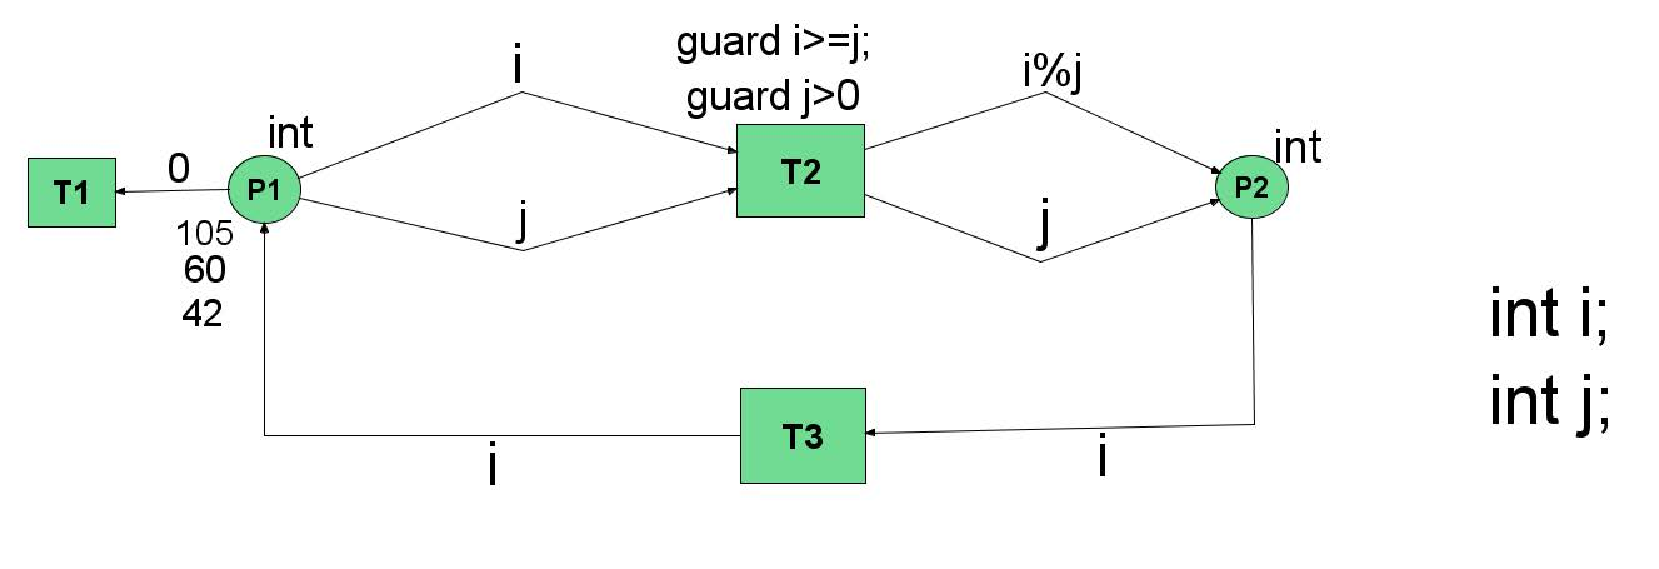
\includegraphics[scale = 0.5]{Comparison_Tools_Renew_Net_GCD.pdf}
	\caption{CPN model to find the GCD of given numbers in Renew}
	\label{fig:Comparison_Tools_Renew_Net_GCD}
\end{figure}


\subsection*{Simulation}
\subparagraph*{\textnormal{Simulation in Renew is interactive. By interactive, we mean to say that the user can choose the enabled transitions to fire along with their bindings. During simulation, the marking of the places are displayed with no explicit feedback of the enabled transitions. However, double clicking on the transition will show if the transition is enabled and one could choose an enabled binding and fire the transition. The markings could also be seen by looking into the simulator log. The screen-shot of the net during simulation along with the simulation traces is given in Figure \ref{fig:Comparison_Tools_Renew_Sim_GCD}. The snapshot of the net is taken at the simulation step 5. In this state, there is a token at place \textit{P1} and 2 tokens at place \textit{P2}. The marking for each step is shown in simulation log. At this state the marking of the place \textit{P1} and \textit{P2} is given by:
\begin{equation*}
\begin{aligned}
m_{P1} =\ & 1^{\backprime}60\\
m_{P2} =\ & 1^{\backprime}3 +\!\!+ 1^{\backprime}42
\end{aligned}
\end{equation*}
Alternatively, one could also see the markings during simulation. The simulation comes to a halt when there are no more enabled transitions. Renew simulator also provides the user with the possibility to play a token game.}}
\begin{figure}[!htbp]
	\centering
	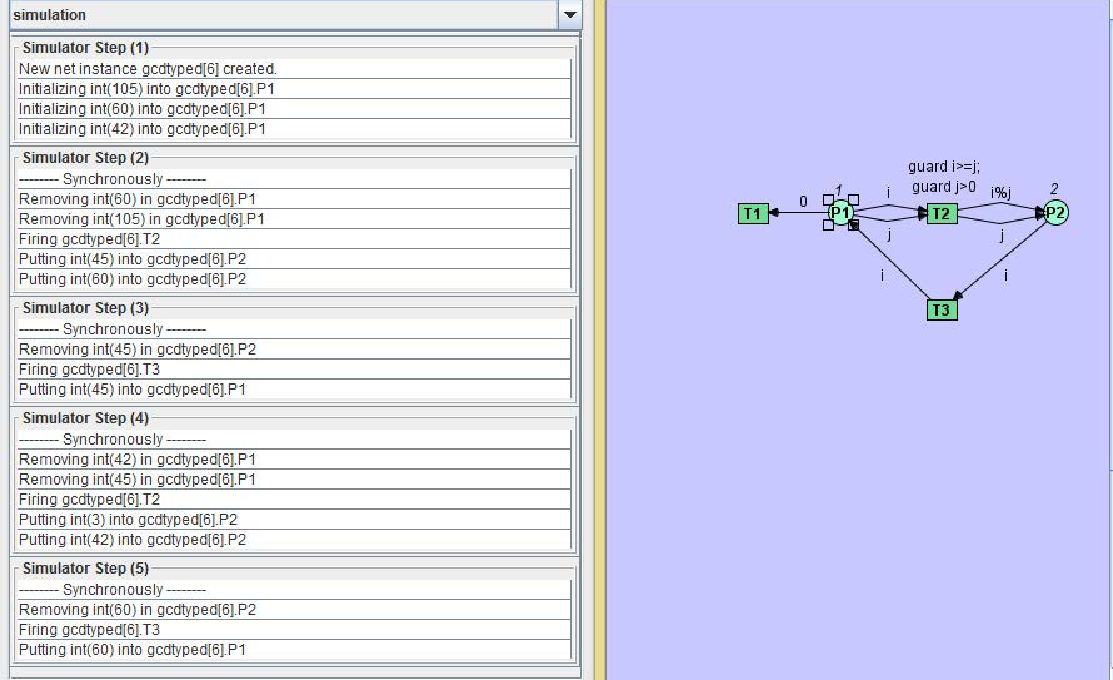
\includegraphics[scale = 0.7]{Comparison_Tools_Renew_Sim_GCD.pdf}
	\caption{Simulation Traces of CPN model in Figure \ref{fig:Comparison_Tools_Renew_Net_GCD}}
	\label{fig:Comparison_Tools_Renew_Sim_GCD}
\end{figure}
\begin{comment}
\subsection{Workflow}
\paragraph*{\textnormal{A short stepwise working of the net is mentioned below:
\begin{enumerate}
\item With the initial marking as 105, 60 and 42, transition $T1$ and $T3$ are disabled (since there are no tokens at place $P2$ and there is no token \bsq{0} at $P1$ for transition to have an enabled binding).
\item There is a non-deterministic choice available for variable $i$ and $j$. Let's suppose that variable $i$ has the binding of 60, in order to satisfy the guard of the transition $T2$, $i \geq j$, $j$ has to be 42. Now with the binding $i$ = 60 and $j$ = 42, $T2$ is fired and the result of $i\%j$ is 18 and the $P2$ has the marking as 18 and 42.
\item Anyone of the tokens present at $P2$ is then transfered to $P1$ (by firing $T3$) and the process is repeated until there are no more enabled transition.
\item When there are no more enabled transitions then the token at $P1$ is counted as the result.
\end{enumerate}}}
\end{comment}

\section{CPN Tools}
\label{sec:app_comp_tools_CPN_Tools}
\paragraph*{\textnormal{According to CPN Tools homepage \cite{CPN_Tools}, CPN Tools is a tool for editing, simulating and analysing Petri net. It was initially developed by the CPN Group at the Aarhus University, Denmark from 2000 to 2010. The main architects behind this tool are Kurt Jensen, S\o ren Christensen, Lars M. Kristensen, and Michael Westergaard. Now the tool has been transferred to the AIS group at Eindhoven University of Technology, The Netherlands.}}

\subparagraph*{\textnormal{CPN Tools has mainly two components namely the graphical editor and the back-end simulator. The graphical editor is written in BETA programming language where as the back-end simulator is written in CPN-ML \cite{CPN_Tools_Extension}. It also has the support for Timed PNs.}}

\subsection*{Modelling}
\subparagraph*{\textnormal{Figure \ref{fig:Comparison_Tools_CPN_Net_GCD} shows the net for calculating the GCD of numbers modelled in CPN Tools. The net structure is almost same as Renew, except the the colour-set definition. In CPN Tools, the colour-sets are defined using CPN-ML as contrary to JAVA syntax in CPN Tools. The work-flow of the net is exactly similar to the net shown in Figure \ref{fig:Comparison_Tools_Renew_Net_GCD}. To model the net, one can use the \textit{Create} palette from the tool box and select the tool under the palette. While selecting a graphical element and using the \bdsq{TAB} key (from the keyboard), one could set different properties for the GUI elements, e.g., guards for transitions, marking of a place, colour-set of a place etc. In CPN-ML one could write guards as the list of boolean expressions. The colour-sets and variables are declared in the declaration section as following:}}
\begin{figure}[!htbp]
	\centering
	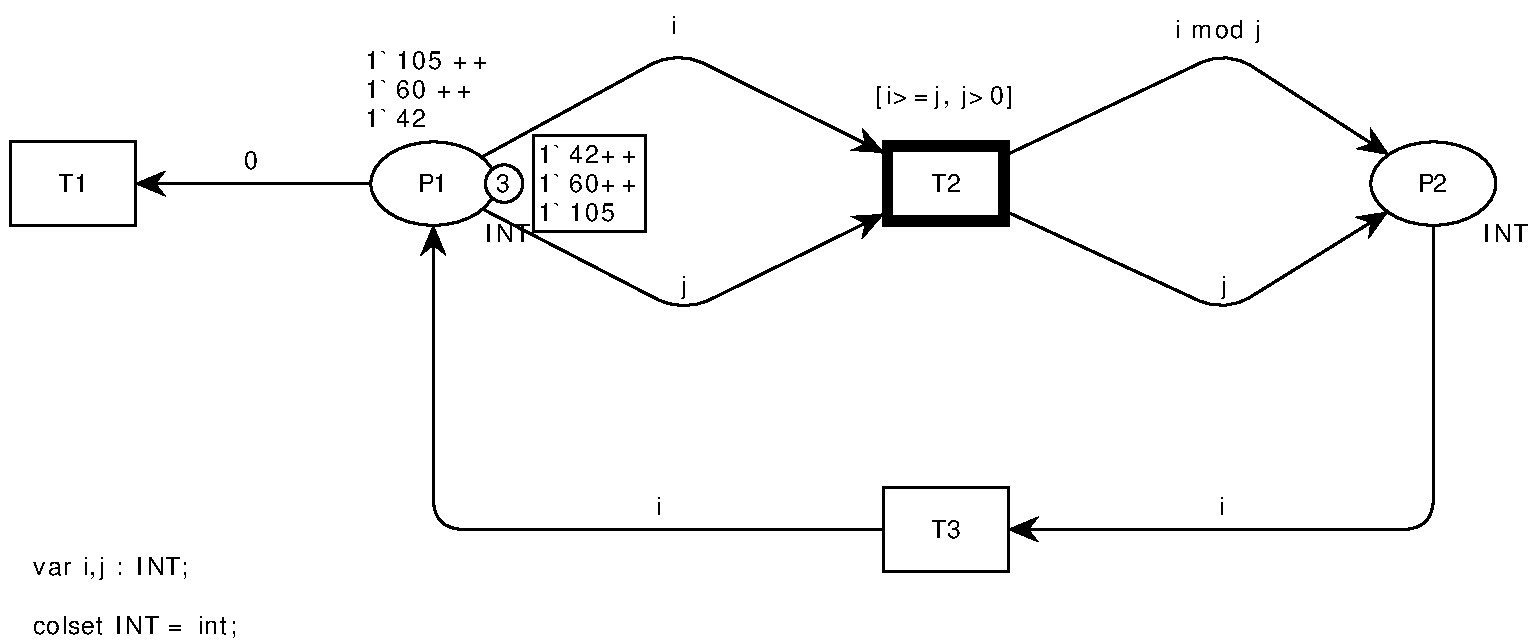
\includegraphics[scale = 0.5]{Comparison_Tools_CPN_Net_GCD.pdf}
	\caption{CPN model to find the GCD of given numbers in CPN Tools}
	\label{fig:Comparison_Tools_CPN_Net_GCD}
\end{figure}
\subparagraph*{title}
\begin{lstlisting}[language = ML, caption = Colour set and variable declaration, captionpos=b, label = lst:colset_var_dec]
COLSET INT = int;
var i,j : INT;
\end{lstlisting}

\subsection*{Simulation}
\subparagraph*{\textnormal{CPN Tools simulator can be found in the \textit{Simulation} palette in the toolbox. There are many ways to simulate the model. One could play the token game an choose bindings manually. One could also limit the number of steps of simulation and allow the simulator to chose the binding non-deterministically. The simulation traces can also be exported as a report to a file. During simulation, the enabled transitions are highlighted \footnote{transitions represented by thick edges, see Figure \ref{fig:Comparison_Tools_CPN_Net_GCD}.}. The markings (during simulation) are represented by the rectangles beside the places.}}
\begin{figure}[!htbp]
	\centering
	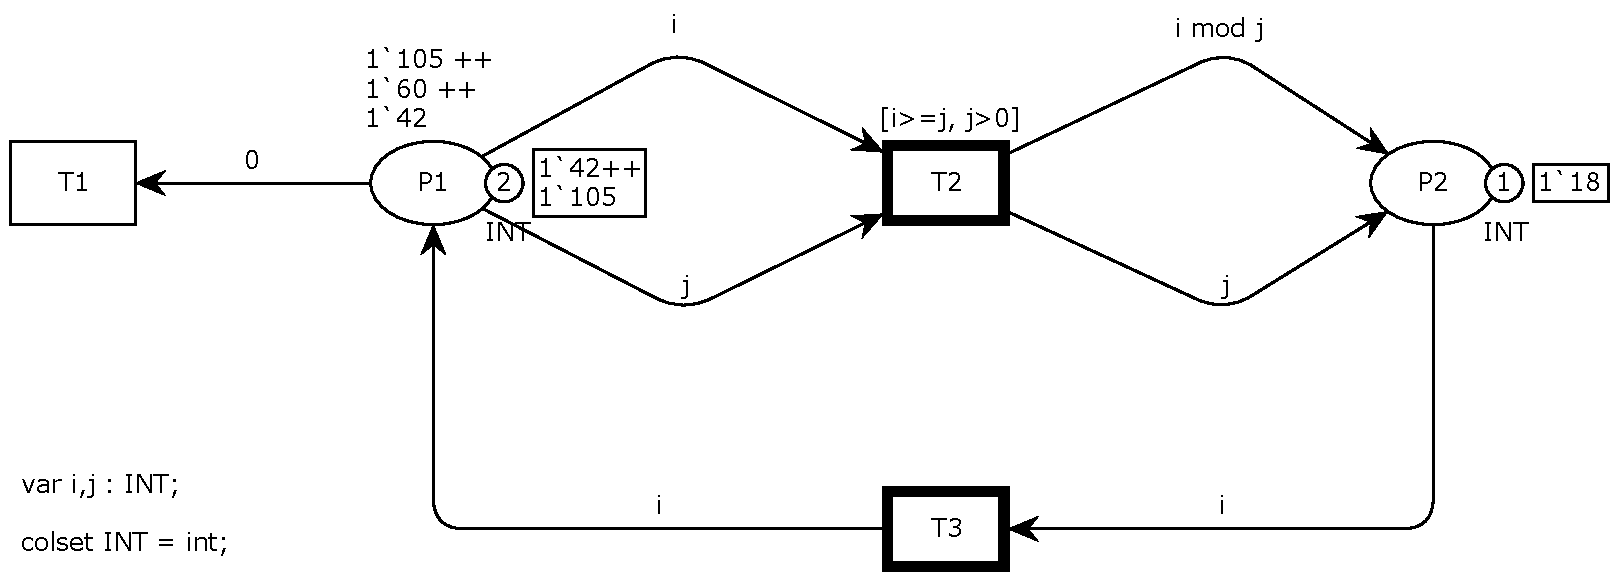
\includegraphics[scale = 0.5]{Comparison_Tools_CPN_Sim_GCD.pdf}
	\caption{Simulation Traces of CPN model in Figure \ref{fig:Comparison_Tools_CPN_Net_GCD}}
	\label{fig:Comparison_Tools_CPN_Sim_GCD}
\end{figure}

\subsection*{Analysis}
\subparagraph*{\textnormal {Contrary to Renew, CPN Tools can also perform analysis on Coloured Petri nets. The tool provides the feature to calculate the state space of the net and analyse its behavioural properties such as liveliness, home markings etc. Analysis of the net is one of the crucial feature and this gives the tool an advantage to get incorporated in academic research and development. The state space graph \footnote{One could refer to the state space graph in section \ref{sec:CPN_Semantics}} for the model in Figure \ref{fig:Comparison_Tools_CPN_Net_GCD} is not shown because it is considerably large.}}

\section{Comparison}
\label{sec:app_comp_tools_comparison}
\paragraph*{\textnormal{We compare these two tools on different parameters and present a justification on the decision of the selection.}}

\subparagraph*{\textnormal{The documentation for Renew is available at \cite{Renew_Homepage} and for CPN Tools is available at \cite{CPN_Tools}. The source code for Renew is freely available at \cite{Renew_Homepage}, where as the source code for CPN Tools is not available. However, some modules of CPN Tools such as \textit{simulator} etc. can be downloaded. A comparison table is shown in the Table \ref{table:Comparison_Tools_Table}. We have considered few factors on which we evaluate both the tools.}}

\begin{table}[!tb]
	\centering
	\begin{tabular}{|c|c|c|}
		\hline
		Features                & Renew                  & CPN Tools       \\ \hline
		Implementation Language & JAVA                   & CPN-ML and BETA \\ \hline
		Platform Supported      & OSX, Windows, Linux 	 & Windows         \\ \hline
		Source Code             & Open Source            & Closed Source   \\ \hline
		Availability            & Free Available         & Free Available  \\ \hline
		Ease of Modelling       & Easy                   & Easy            \\ \hline
		Easy of Simulation      & Easy                   & Easy            \\ \hline
		Analysis                & Not Supported          & Supported       \\ \hline
		Debugger Support        & Yes                    & Yes             \\ \hline
		Extensibility           & Yes                    & Yes             \\ \hline
		Latest Version			& 2.5					 & 4.0.1			\\ \hline
	\end{tabular}
	\caption{Comparison Table}
	\label{table:Comparison_Tools_Table}
\end{table}

\subparagraph*{\textnormal{Renew gains advantage in most of the mentioned features. One such feature is its implementation language, JAVA, which is a very well known language in contrast to CPN-ML and BETA which is used by CPN Tools. Development in one of the well known programming language is easier. However, CPN Tools has exposed its APIs, through Access/CPN \cite{AccessCPN_Library}, in JAVA for developing extensions. Further, Renew is supported more known platforms such as Linux, OSX and even its experimental version of android exists. However, the major reason for our selection of CPN Tools over Renew is its wide use in industry along with its support for analysis of CP-nets.}}

\subparagraph*{\textnormal{For our purpose, we want to model non-hierarchical Coloured Petri nets and perform analysis of the net. Renew also supports modelling of non-hierarchical Coloured Petri nets but it does not support analysis. Renew can be a good contender in future for developing extensions once it starts supporting analysis over CP-nets.}}

